{ %section1_6
	\subsection{The main approaches to parallelization}
	\par In practice, there are a large number of parallel computing patterns. However, all these patterns basically use three basic approaches to parallelization:
	\begin{itemize}
		\item\textbf{Data parallelization:} The programmer finds in the program an array of data whose elements the program sequentially processes in some func function. Then the programmer tries to break this data array into blocks that can be processed in func independently of each other. Then the programmer starts several threads at once, each of which executes func, but at the same time processes data blocks different from other flows in this function.
		\item\textbf{Instruction parallelization:} The programmer finds in the program sequentially called functions, the process of which does not affect each other (such functions do not change common global variables, and the results of one are not used by the other). Then the programmer starts these functions in parallel threads.
		\item\textbf{Parallelization of information flows:} A program is a set of functions that can be performed, and several functions can expect the result of the previous ones. In this case, each core performs the function for which the data is already ready. Consider this method as an example of an abstract dual-core processor, as the most difficult to understand. The structural algorithm shown in Figure~\ref{structAlgorithm:image} consists of 9 functions, some of which use the result of the previous function in their work. We assume that function 3 uses the result of the function 1, and function 7 uses the result of functions 4 and 6, etc., and also function 5 is executed in time approximately as much as functions 7, 8, and 9 combined. Then, on a dual-core machine, this parallelization method will be the optimal solution.
	\end{itemize}
	\begin{figure}[H]
		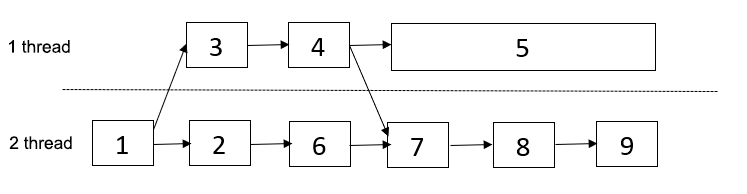
\includegraphics[width=1\linewidth]{structAlgorithm}
		\caption{\textit{An example of the operation of a structural \\algorithm on a dual-core processor}}
		\label{structAlgorithm:image}
	\end{figure}
	\par The three methods described are easier to understand by analogy from everyday life. Let two students in the construction team be given the task of sweeping the street and painting the fence. If students decide to use data parallelization, he will first sweep the street together, and then paint the fence together. If they decide to use parallelization according to the instructions, then one student will completely sweep the street, and the other will paint the entire fence at this time. This situation cannot be parallelized over the information flows, since these two actions are in no way dependent on each other. If we assume that they both need tools for work, then one of them must first go after them, and then both of them will begin to do their work.
	\par In more cases, the decision to use the method is obvious due to the internal features of the parallelized program. The choice of method is determined by which one loads flows more evenly. Ideally, all threads should finish the work allocated to them approximately at the same time in order to optimally load the kernels (processors) and so that the threads that have finished their work do not stand idle while waiting for the completion of work by neighboring threads.
	\par
}
